%% 
%% Copyright 2007-2024 Elsevier Ltd
%% 
%% This file is part of the 'Elsarticle Bundle'.
%% ---------------------------------------------
%%  
%% It may be distributed under the conditions of the LaTeX Project Public
%% License, either version 1.3 of this license or (at your option) any%% later version.  The latest version of this license is in
%%    http://www.latex-project.org/lppl.txt
%% and version 1.3 or later is part of all distributions of LaTeX
%% version 1999/12/01 or later.
%% 
%% The list of all files belonging to the 'Elsarticle Bundle' is
%% given in the file `manifest.txt'.
%% 
%% Template article for Elsevier's document class `elsarticle'
%% with harvard style bibliographic references

\documentclass[preprint,12pt,authoryear]{elsarticle}

%% Use the option review to obtain double line spacing
%% \documentclass[authoryear,preprint,review,12pt]{elsarticle}

%% Use the options 1p,twocolumn; 3p; 3p,twocolumn; 5p; or 5p,twocolumn
%% for a journal layout:
%% \documentclass[final,1p,times,authoryear]{elsarticle}
%% \documentclass[final,1p,times,twocolumn,authoryear]{elsarticle}
%% \documentclass[final,3p,times,authoryear]{elsarticle}
%% \documentclass[final,3p,times,twocolumn,authoryear]{elsarticle}
%% \documentclass[final,5p,times,authoryear]{elsarticle}
%% \documentclass[final,5p,times,twocolumn,authoryear]{elsarticle}

\usepackage{standalone}
\usepackage{pgf}
\usepackage{pgfkeys}
\usepackage{gnuplottex}
\usepackage{gnuplot-lua-tikz}

\renewcommand{\figurename}{\textbf{Fig}}

%% For including figures, graphicx.sty has been loaded in
%% elsarticle.cls. If you prefer to use the old commands
%% please give \usepackage{epsfig}
%% The amssymb package provides various useful mathematical symbols
\usepackage{amssymb}
\usepackage{graphicx}
%% The amsmath package provides various useful equation environments.
\usepackage{amsmath}
\usepackage{algorithm}
\usepackage{algorithmicx}
\usepackage{algpseudocode}
\usepackage{pgfplots}
\usepackage{epstopdf}  % Automates EPS to PDF conversion
%% The amsthm package provides extended theorem environments
%% \usepackage{amsthm}

% Sets
\newcommand{\SetWorkOrder}[1]{W(\VarMetaTime#1)}
\newcommand{\ElementWorkOrder}{w}
\newcommand{\SetPeriod}{P(\VarMetaTime)}
\newcommand{\ElementPeriod}{p}

\newcommand{\SetResource}{R(\VarMetaTime)}
\newcommand{\ElementResource}{r}
\newcommand{\SetOperation}[2]{O_{#1}(\VarMetaTime, #2)}
\newcommand{\ElementOperation}{o}

\newcommand{\SetDays}[1]{D_{#1}(\VarMetaTime)}
\newcommand{\ElementDays}{d}
\newcommand{\SetActivity}[2]{A_{#2}(\VarMetaTime, #1)}
\newcommand{\ElementActivity}{a}

\newcommand{\SetWorkSegment}{K(\VarSupervisorAssignment{}{})}
\newcommand{\ElementWorkSegment}{k}
\newcommand{\SetTimeInstance}{I(\VarMetaTime)}
\newcommand{\ElementTimeInstance}{i}

\newcommand{\SetEvent}{E(\VarMetaTime)}
\newcommand{\ElementEvent}{e}

\newcommand{\SetScheduler}{S}
\newcommand{\ElementScheduler}{s}
\newcommand{\SetSupervisor}{Z}
\newcommand{\ElementSupervisor}{z}

\newcommand{\SetTechnician}{T(\VarMetaTime)}
\newcommand{\ElementTechnician}{t}

% Parameters
\newcommand{\ParStrategicValue}{strategic\_value_{\ElementWorkOrder \ElementPeriod}(\VarMetaTime)}
\newcommand{\ParStrategicPenalty}{strategic\_penalty}
\newcommand{\ParClusteringValue}{clustering\_value_{\ElementWorkOrder1, \ElementWorkOrder2}}
\newcommand{\ParStrategicResource}{resource_{\ElementPeriod\ElementResource}(\VarMetaTime)}

\newcommand{\ParStrategicWorkOrderWeight}{work\_order\_work_{\ElementWorkOrder \ElementResource}}
\newcommand{\ParStrategicInclude}{include(\VarMetaTime)}
\newcommand{\ParStrategicExclude}{exclude(\VarMetaTime)}
\newcommand{\ParTacticalValue}{tactical\_value_{\ElementDays\ElementOperation}(\VarMetaTime)}

\newcommand{\ParTacticalPenalty}{tactical\_penalty}
\newcommand{\ParOperationWork}[1]{work_{#1}(\VarMetaTime)}
\newcommand{\ParTacticalResource}{tactical\_resource_{\ElementDays\ElementResource}(\VarMetaTime)}
\newcommand{\ParStartStart}{start\_start_{\ElementOperation1, \ElementOperation2}}

\newcommand{\ParFinishStart}{finish\_start_{\ElementOperation1, \ElementOperation2}}
\newcommand{\ParEarliestStart}{earliest\_start_{\ElementOperation}(\VarMetaTime)}
\newcommand{\ParLatestFinish}{latest\_finish_{\ElementOperation}(\VarMetaTime)}
\newcommand{\ParNumberOfPeople}{number_{\ElementOperation}(\VarMetaTime)}

\newcommand{\ParOperatingTime}{operating\_time_{\ElementOperation}}
\newcommand{\ParDuration}{duration_{\ElementOperation}(\VarMetaTime)}
\newcommand{\ParSupervisorValue}{supervisor\_value_{\ElementActivity \ElementTechnician}(\VarMetaTime, \VarStartOfSegment{t}{}, \VarFinishOfSegment{t}{})} 
\newcommand{\ParFeasible}{feasible_{at}(\VarIncludeActivity{})}
\newcommand{\ParOperationsForWorkOrder}{work\_order\_to\_operations_{\ElementWorkOrder }}

\newcommand{\ParOperationsInWorkOrder}{operations\_in\_work\_order_{\ElementWorkOrder }}
\newcommand{\ParActivitiesForOperation}{activities\_for\_operation_{\ElementOperation}}
\newcommand{\ParLowerActivityWork}{lower\_activity\_work_{\ElementActivity}(\VarMetaTime)}
\newcommand{\ParActivityWork}[1]{activity\_work_{\ElementActivity}(\VarMetaTime, \VarActivityWork{#1})}

\newcommand{\ParPreparation}{preparation_{\ElementActivity1, \ElementActivity2}}
\newcommand{\ParEvent}{event_{\ElementTimeInstance \ElementEvent}}
\newcommand{\ParEventDuration}{duration_{\ElementTimeInstance \ElementEvent}}
\newcommand{\ParConstraintLimit}{constraint\_limit}

\newcommand{\ParTimeWindowStart}{time\_window\_start_{\ElementActivity}(\VarTacticalWork{}{})}
\newcommand{\ParTimeWindowFinish}{time\_window\_finish_{\ElementActivity}(\VarTacticalWork{}{})}
\newcommand{\ParAvailabilityStart}{availability\_start(\VarMetaTime)}
\newcommand{\ParAvailabilityFinish}{availability\_finish(\VarMetaTime)}

% Variables
\newcommand{\VarStrategicWorkOrderAssignment}[2]{\alpha_{#1#2}(\VarMetaTime)}
\newcommand{\VarStrategicExcess}{\epsilon_{\ElementPeriod\ElementResource}(\VarMetaTime)}
\newcommand{\VarTacticalWork}[2]{\beta_{#1#2}(\VarMetaTime)}
\newcommand{\VarTacticalExcess}{\mu_{\ElementResource \ElementDays}(\VarMetaTime)} 

\newcommand{\VarTacticalWorkBinary}[2]{\sigma_{#1#2}(\VarMetaTime)}
\newcommand{\VarTacticalWorkBinaryConsecutive}{\eta_{\ElementDays\ElementOperation}(\VarMetaTime)}
\newcommand{\VarTacticalOperationDifference}{\Delta_{\ElementOperation}(\VarMetaTime)}
\newcommand{\VarSupervisorAssignment}[2]{\gamma_{#1#2}(\VarMetaTime)}

\newcommand{\VarSupervisorAssignmentWhole}{\phi_{\ElementOperation}(\VarMetaTime)}
\newcommand{\VarActivityWork}[1]{\rho_{#1}(\VarMetaTime)}
\newcommand{\VarProcessingTime}{\delta_{\ElementActivity\ElementWorkSegment}(\VarMetaTime)} 
\newcommand{\VarActiveSegment}[2]{\pi_{#1#2}(\VarMetaTime)}

\newcommand{\VarStartOfSegment}[2]{\lambda_{#1#2}(\VarMetaTime)}
\newcommand{\VarFinishOfSegment}[2]{\Lambda_{#1#2}(\VarMetaTime)}
\newcommand{\VarSegmentInRelation}{\omega_{\ElementActivity\ElementWorkSegment\ElementTimeInstance \ElementEvent}(\VarMetaTime)}
\newcommand{\VarIncludeActivity}[1]{\theta_{#1}(\VarMetaTime)}

% Meta variables
\newcommand{\VarMetaTime}{\tau}


\definecolor{red}{HTML}{8A3F3A}
\definecolor{yellow}{HTML}{E0BB3C}
\definecolor{blue}{HTML}{4569E0}
\definecolor{green}{HTML}{17E561}
\definecolor{other}{HTML}{6A939E}

% DTU Colors
\definecolor{dtu-corporate-red}{HTML}{990000}
\definecolor{dtu-white}{HTML}{ffffff}
\definecolor{dtu-black}{HTML}{000000}
\definecolor{dtu-blue}{HTML}{2F3EEA}
\definecolor{dtu-bright-green}{HTML}{1FD082}
\definecolor{dtu-navy-blue}{HTML}{030F4F}
\definecolor{dtu-yellow}{HTML}{F6D04D}
\definecolor{dtu-orange}{HTML}{FC7634}
\definecolor{dtu-pink}{HTML}{F7BBB1}
\definecolor{dtu-grey}{HTML}{DADADA}
\definecolor{dtu-red}{HTML}{E83F48}
\definecolor{dtu-green}{HTML}{008835}
\definecolor{dtu-purple}{HTML}{79238E}

\usepackage[utf8]{inputenc}
\usepackage[T1]{fontenc}
\usepackage{graphicx}
\usepackage{amsmath}
\usepackage{makecell}
\usepackage{amssymb}
\usepackage{multicol}
\usepackage{natbib}
\usepackage{hyperref}
\usepackage{booktabs} % For professional quality tables
\usepackage{array}    % For better column alignment
\usepackage{tikz}
\usepackage{pgfkeys}
%% The lineno packages adds line numbers. Start line numbering with
%% \begin{linenumbers}, end it with \end{linenumbers}. Or switch it on 
%% for the whole article with \linenumbers.
%% \usepackage{lineno}

\journal{Journal of Scheduling}

\begin{document}

\begin{frontmatter}

%% Title, authors and addresses

%% use the tnoteref command within \title for footnotes;
%% use the tnotetext command for theassociated footnote;
%% use the fnref command within \author or \affiliation for footnotes;
%% use the fntext command for theassociated footnote;
%% use the corref command within \author for corresponding author footnotes;
%% use the cortext command for theassociated footnote;
%% use the ead command for the email address,
%% and the form \ead[url] for the home page:
%% \title{Title\tnoteref{label1}}
%% \tnotetext[label1]{}
%% \author{Name\corref{cor1}\fnref{label2}}
%% \ead{email address}
%% \ead[url]{home page}
%% \fntext[label2]{}
%% \cortext[cor1]{}
%% \affiliation{organization={},
%%            addressline={}, 
%%            city={},
%%            postcode={}, 
%%            state={},
%%            country={}}
%% \fntext[label3]{}

\title{Optimizing a Maintenance Scheduling System Through the Use of Atomic Pointer Swap} %% Article title

%% use optional labels to link authors explicitly to addresses:
%% \author[label1,label2]{}
%% \affiliation[label1]{organization={},
%%             addressline={},
%%             city={},
%%             postcode={},
%%             state={},
%%             country={}}
%%
%% \affiliation[label2]{organization={},
%%             addressline={},
%%             city={},
%%             postcode={},
%%             state={},
%%             country={}}

\author[DTUconstruct]{Christian Brunbjerg Jespersen} %% Author name
\author[DTUconstruct]{Kristoffer Sigsgaard Wernblad}
\author[DTUmanagement]{Thomas Jacob Riis Stidsen}
\author[DTUconstruct]{Kasper Barslund Hansen}
\author[DTUconstruct]{Jingrui Ge}
\author[DTUconstruct]{Simon Didriksen}
\author[DTUconstruct]{Niels Henrik Mortensen}

%% Author affiliation
\affiliation[DTUconstruct]{organization={DTU Construct, Technical University of Denmark},%Department and Organization
            addressline={Anker Egelundsvej 1}, 
            city={Kongens Lyngby},
            postcode={2800}, 
            state={Hovedstaden},
            country={Denmark}}
\affiliation[DTUmanagement]{organization={DTU Management, Technical University of Denmark},%Department and Organization
            addressline={Anker Egelundsvej 1}, 
            city={Kongens Lyngby},
            postcode={2800}, 
            state={Hovedstaden},
            country={Denmark}}

%% Abstract
\begin{abstract}
            
\end{abstract}

%%Graphical abstract
%\begin{graphicalabstract}
%\includegraphics{grabs}
%\end{graphicalabstract}

%%Research highlights
%\begin{highlights}
%\item How to allow direct and real-time integration into an optimization process?
%\item How to perform optimization in a real-time changing parameter space?
%\end{highlights}

%% Keywords
\begin{keyword}
%% keywords here, in the form: keyword \sep keyword
Large Neighborhood Search
\sep\ Actor Framework
\sep\ Maintenance scheduling
\sep\ Real-time Optimization
\sep\ Human-centered Computing
\sep\ Decision Support Systems
\sep\ Concurrent Software Architecture
%% PACS codes here, in the form: \PACS code \sep code

%% MSC codes here, in the form: \MSC code \sep code
%% or \MSC[2008] code \sep code (2000 is the default)
\end{keyword}

\end{frontmatter}

\section{Introduction}
Maintenance scheduling is part of a class of operational problems that
have proven hard to solve in practice (maintenance scheduling problems are usually modelled as
resource-constrained project scheduling problems, knapsack formulations,
machine scheduling problems, etc.\ which are all NP-hard problems~\citep{garey1979computers}).
To be effective in dynamic and uncertain environments where maintenance
scheduling is carried out, optimization must be tightly integrated with
existing IT infrastructure. This integration ensures that the tacit knowledge of
decision-makers can seamlessly influence the planning process.
The planning process often involves multiple decision-makers operating at
different business levels. As a result, responsibility for decision-making is
typically assigned to individuals who represent only a small segment of the
overall process.
These multiple smaller planning processes are often difficult to map to
a single mathematical model describing the whole system as elaborated
by~\citep{barthelemy2002human}. Solving operation research problems that
are operational in nature have additional requirements over more typical
static problems: they have to be responsive to changing parameters; able to
be assimilated into the decision-makers workflow; allow for integration with
dynamic data sources such as databases and APIs~\citep{meignan_review_2015}.
Operational aspects of operation research, as opposed to higher level
strategic and tactical ones, are characterized by extensive amounts
coordination and negotiation on proposed schedules often in a short amount of
time~\citep{palmerMaintenancePlanningScheduling2019}.

The lack of integration into the schedulers and supervisors workflow
and lack of responsiveness can lead to a situation where solutions are
not directly implemented in practice but instead only provides initial
suggestions~\citep{meignan_review_2015}. Theses initial suggestions are then
iterated on elsewhere in the scheduling process usually through much more manual
means. In~\citep{barthelemy2002human} the authors argue that many problems that
operation research aim to solve are often composed of a group of individuals
whose decisions are consolidated into an ``epistemic subject'' for which a
mathematical model can be formulated and solved, with many scheduling problems
being good examples. However, often multiple actors have different views on what
constitutes an optimal schedule hence resulting in multiple-objectives. Even if
multi-objective optimization~\citep{ehrgott2002multiple} is applied to find a
Pareto Front~\citep{Pareto1897} a negotiating process still is needed between
the actors to select the final schedule.

This paper proposes a solution method that will allow for real-time optimization
based on actor/user interaction and a connection to a dynamic data source,
effectively managing the changes to the parameter space as they occur. The
proposed solution method will be tested on the weekly maintenance scheduling
problem \citep{palmerMaintenancePlanningScheduling2019weeklyscheduling}
which closely resembles a variant of the multi-compartment multi-knapsack
problem (MCMKP)~\citep{do2007constrained}. It should be noted
that the scientific maintenance scheduling literature can deviate
significantly from its practical implementation which is detailed in
\citep{palmerMaintenancePlanningScheduling2019}. The solution method is based
on the large neighborhood search (LNS~\citep{shaw1998using}) metaheuristic and
is in this paper described as actor-based large neighborhood search (AbLNS). LNS
was chosen due to its properties of naturally being able to work with and fix
infeasible solutions and because of its state of the art performance on various
scheduling problems \citep{gendreauHandbookMetaheuristics2019lnschapter}.
% TODO Find a better source for the LNS performance.

To understand the need for actor-based methods some
background knowledge will be required about the maintenance scheduling process.
Figure~\ref{fig:integrated:maintenance-process} illustrates the general setup
of a maintenance planning and scheduling system. The system's actors
have the following responsibilities: the planner generates the work orders that
are to be scheduled; each scheduler creates weekly schedules for a set of work orders; 
based on the weekly schedule the supervisors assign work order
activities to technicians; the
technicians executes the work. Each planning problem is matched 
by a corresponding optimization problem, for the scheduler, it is a variation of the
multi-compartment multi-knapsack problem, for the supervisor it is a variation of the 
assignment problem and for the technicians it is a single machine scheduling problem.

The concept of ``ownership'' of a work order is fundamental to understanding
the need for actor-based approaches. During the scheduling process, each work
order is assigned to a specific actor, who alone has the authority to modify or
execute it.

This means that a single model approach is very difficult to implement in practice
as a work order is modelled differently depending on the actor that currently
owns it. This highlights another point in maintenance scheduling: that
the stochastic nature of the maintenance scheduling process can be handled using
a change of model, each with different levels of aggregation and different sets
of constraints, opposed to more academic approaches such as fuzzy logic and
stochastic optimization. When the inherrent uncertainties manifest themselves
during planning or execution, work orders are rescheduled by moving between
the different actors, meaning that the stochastic elements of maintenance
scheduling are handled by \textbf{dynamic rescheduling between the actors}.

\begin{figure}
	\usetikzlibrary{positioning}
\definecolor{red}{HTML}{8A3F3A}
\definecolor{yellow}{HTML}{E0BB3C}
\definecolor{blue}{HTML}{4569E0}
\definecolor{green}{HTML}{17E561}
\definecolor{other}{HTML}{6A939E}

% DTU Colors
\definecolor{dtu-corporate-red}{HTML}{990000}
\definecolor{dtu-white}{HTML}{ffffff}
\definecolor{dtu-black}{HTML}{000000}
\definecolor{dtu-blue}{HTML}{2F3EEA}
\definecolor{dtu-bright-green}{HTML}{1FD082}
\definecolor{dtu-navy-blue}{HTML}{030F4F}
\definecolor{dtu-yellow}{HTML}{F6D04D}
\definecolor{dtu-orange}{HTML}{FC7634}
\definecolor{dtu-pink}{HTML}{F7BBB1}
\definecolor{dtu-grey}{HTML}{DADADA}
\definecolor{dtu-red}{HTML}{E83F48}
\definecolor{dtu-green}{HTML}{008835}
\definecolor{dtu-purple}{HTML}{79238E}


\newlength{\basisa}
\setlength{\basisa}{1cm}
\centering
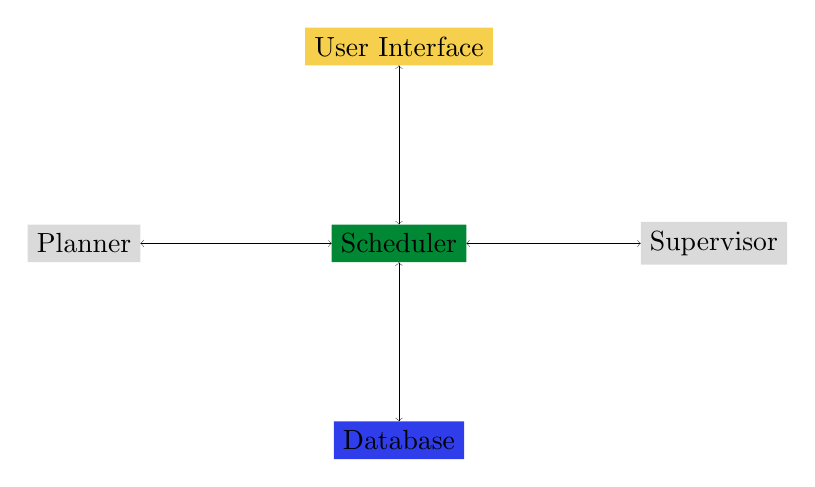
\begin{tikzpicture}[line width=0.0\basisa]
    \draw (4.0\basisa,4.0\basisa) 
		node[minimum height=2\basisa,fill=dtu-grey,minimum width=3\basisa,rounded corners=0.1\basisa] 
			(Planner) {Planner};
    \draw (12.0\basisa,4.0\basisa) 
		node[minimum height=2\basisa,fill=dtu-grey,minimum width=3\basisa,rounded corners=0.1\basisa] 
			(Supervisor) {Supervisor};

			
    \draw (8.0\basisa,4.0\basisa) 
		node[minimum height=2\basisa,fill=dtu-green,minimum width=3\basisa,rounded corners=0.1\basisa] 
			(Scheduler) {Scheduler};
	
    \draw (8.0\basisa,1.5\basisa) 
		node[minimum height=1\basisa,fill=dtu-blue,minimum width=3\basisa,rounded corners=0.1\basisa] 
			(Database) {Database};

    \draw (8.0\basisa,6.5\basisa) 
		node[minimum height=1\basisa,fill=dtu-yellow,minimum width=3\basisa,rounded corners=0.1\basisa] 
			(UserInterface) {User Interface};

	\draw[<->, thick, line width=0.1\basisa] (Planner) -- (Scheduler);
	\draw[<->, thick, line width=0.1\basisa] (Scheduler) -- (Supervisor);
	\draw[<->, thick, line width=0.1\basisa] (Scheduler) -- (Database);
	\draw[<->, thick, line width=0.1\basisa] (Scheduler) -- (UserInterface);
\end{tikzpicture}

	\caption{Simple overview of a maintenance scheduling process with its primary types of
		actors. The planner, the scheduler, the supervisor(s), and the technicians. 		
		The green color highlights the scheduler as it the actor in the maintenance
		scheduling process that is modelled in this paper.
	}\label{fig:integrated:maintenance-process}
\end{figure}

The primary contribution of this article is the development of a modular,
scalable optimization component. This component leverages a proven metaheuristic
to support business processes constructed from smaller mathematical models
within a framework, rather than relying on a single, integrated mathematical
model.

The paper is organized into four sections. Section~\ref{sec:2-solution-method}
provides a detailed explanation of the weekly maintenance scheduling model,
which serves as the foundation of the study. Section~\ref{sec:3-results}
presents the results obtained from the implemented metaheuristic, highlighting
its response to simulated user interactions. Section~\ref{sec:4-discussion}
discusses the research implications and outlines potential directions for
future work. While all source code for the implemented system is available at
\citep{scipo-code-ordinator_api}, the instance data remains confidential and
cannot be shared publicly.

\subsection{The Weekly (Period) Maintenance Scheduling Model}
The weekly maintenance scheduling model for the problem is a variant of
the Multi-compartment Multi-knapsack Problem with capacity penalties MCMKP\@
The notation used to describe the dynamical aspects in the model is based
on the notation from the dynamic metaheuristics literature as found 
in~\citep{yangMetaheuristicsDynamicCombinatorial2013}. % TODO: Is there a better source
source on the dynamic notation. Here $\VarMetaTime$ is added as a time variable
on all sets, parameters, and variables that are subject to change while the
metaheuristic is running. This enables precise timing on the messages that
are send to the AbLNS and understand how it reacts in real-time. A company
performing maintenance usually creates weekly maintenance plans for the
next $\ElementPeriod \in \SetPeriod$ period. The weekly schedule is created
centrally and consists of scheduling the $\ElementWorkOrder \in \SetWorkOrder$
work orders, i.e.\ maintenance tasks, such that all $\ElementWorkOrder$
are scheduled into a specific period $\ElementPeriod$. Each work order $
\ElementWorkOrder$ requires some resources $\ElementResource \in \SetResource$
to be carried out, e.g.\ man-power with different qualifications. Each of these
resources are available in limited amounts given by $\ParStrategicResource$.
To correct for possible manual interventions that can make the problem
infeasible a penalty ($\ParStrategicResourcePenalty$) is introduced.
The urgency of the different maintenance work order ($\ElementWorkOrder$)
varies and is reflected in a `tardiness' for carrying out a maintenance
work order in a certain period given by $\ParStrategicUrgency$. The $
\ParStrategicUrgency$ also captures the tardiness of the individual work orders
($\ElementWorkOrder$), meaning that the value gained from scheduling work
orders late is increasing. Urgent tasks have increasing value the further out
the period $\ElementPeriod$ becomes. Furthermore, two sets exists which will
either require work order $\ElementWorkOrder$ to be carried out in period $
\ElementPeriod$ or not carried out in a period $\ElementPeriod$. These sets are
$(\ElementWorkOrder,\ElementPeriod) \in \ParStrategicInclude$ for inclusion and
$(\ElementWorkOrder, \ElementPeriod) \in \ParStrategicExclude$ for exclusion.


\newpage
\begin{alignat}{2}
	& \text{\rule{\linewidth}{0.4pt}} \notag\\
	& \textbf{Meta variables:} \notag\\
	& \ElementScheduler \in \SetScheduler \\
	& \VarTacticalWork{}{} \\ 
	& \tau \in [0, \infty] \\
	& \text{\rule{\linewidth}{0.4pt}} \notag\\
	& \textbf{Minimize:} \notag                                                                                                                                                        \\
	& \sum_{\ElementWorkOrder \in \SetWorkOrder{}} \sum_{\ElementPeriod \in \SetPeriod} \ParStrategicValue \cdot \VarStrategicWorkOrderAssignment{\ElementWorkOrder}{\ElementPeriod}  \notag\\ 
	& + \sum_{\ElementPeriod \in \SetPeriod} \sum_{\ElementResource \in \SetResource} \ParStrategicPenalty \cdot \VarStrategicExcess     \notag                                              \\
	& + \sum_{\ElementPeriod \in \SetPeriod} \sum_{\ElementWorkOrder1 \in \SetWorkOrder{}} \sum_{\ElementWorkOrder2 \in \SetWorkOrder{}} 	 \quad \ParClusteringValue \cdot \VarStrategicWorkOrderAssignment{\ElementWorkOrder1}{\ElementPeriod} \cdot \VarStrategicWorkOrderAssignment{\ElementWorkOrder2}{\ElementPeriod}  \\
	& \text{\rule{\linewidth}{0.4pt}} \notag\\
	& \textbf{Subject to:} \notag                                                                                                                                                      \\
	& \sum_{\ElementWorkOrder \in \SetWorkOrder{}} \ParStrategicWorkOrderWeight \cdot \VarStrategicWorkOrderAssignment{\ElementWorkOrder}{\ElementPeriod} \leq \ \ParStrategicResource + \VarStrategicExcess                                                                           \quad \forall \ElementPeriod \in \SetPeriod \quad \forall \ElementResource \in \SetResource                                                                                      \\
	& \sum_{\ElementWorkOrder \in \SetWorkOrder{}} \VarStrategicWorkOrderAssignment{\ElementWorkOrder}{\ElementPeriod} = 1              \quad \forall \ElementPeriod \in \SetPeriod                                                                                                                                      \\
	& \VarStrategicWorkOrderAssignment{\ElementWorkOrder}{\ElementPeriod} = 0                                                            \quad \forall (\ElementWorkOrder, \ElementPeriod) \in \ParStrategicExclude                                                                                                       \\
	& \VarStrategicWorkOrderAssignment{\ElementWorkOrder}{\ElementPeriod} = 1                                                            \quad \forall (\ElementWorkOrder, \ElementPeriod) \in \ParStrategicInclude                                                                                                       \\
	& \VarStrategicWorkOrderAssignment{\ElementWorkOrder}{\ElementPeriod} \in \{0, 1\}                                                   \quad \forall \ElementWorkOrder \in \SetWorkOrder{} \quad \forall \ElementPeriod \in \SetPeriod                                                                                 \\ 
	& \VarStrategicExcess \in \mathbb{R}^{+}                                                                                             \quad \forall \ElementPeriod \in \SetPeriod \quad \forall \ElementResource \in \SetResource                                                                                  \\ 
	& \text{\rule{\linewidth}{0.4pt}} \notag
\end{alignat}
\newpage


\strategicmodel[clustering=true, beta=false]

The meta variables defines the broader setting that the model in implemented in.
Equation~\eqref{eqn:meta:scheduler:strategic} specicies that the model is
implemented for scheduler \ElementScheduler. 
Equation~\eqref{eqn:meta:time:strategic} is the time variable that binds the whole
system together, by allowing us to reason about the sequence that events are 
happening in.

The objective function~\eqref{eqn:objective:strategic}, minimizes the
total weighted assignment of all work orders subtracted by the penalty $
\ParStrategicResourcePenalty$ for exceeding the resource capacity given in
equation~\eqref{eqn:strategic:constraint:resource}. The third term of the
objective function handles the $\ParClusteringValue$ which turns the model into
a quadratic problem. This term optimizes the value of scheduling two work orders
in the same period, if they have share similarity like close proximity, same
piece/type of equipment, etc. Equation~\eqref{eqn:strategic:constraint:resource}
ensures that all the $\ParOperationWork{wr}$ for each activity in
a work order, given that it has been assigned, is lower than the $
\ParStrategicResource$ for each $\ElementPeriod$ and for each resources $
\ElementResource$. $\ParStrategicResourcePenalty$ is the amount of exceeded
capacity that is needed for the current assignment of work orders to be
feasible. Equation~\eqref{eqn:constraint:strategic:schedule_once} makes
sure that each work order is assigned to at least a one period. 
Equation~\eqref{eqn:strategic:constraint:exclude} excludes a work order from a
certain period and equation~\eqref{eqn:constraint:strategic:include}
forces a specific work order to be included in a specific
period. Constraint~\eqref{eqn:variable:strategic:assignment} 
and~\eqref{eqn:variable:strateigc:penalty} specify the variable domain for $
\VarStrategicWorkOrderAssignment{\ElementWorkOrder}{\ElementPeriod}$ and
$ \ParStrategicResourcePenalty$ respectively. The effects of changing $
\ParStrategicInclude$, $\ParStrategicExclude$, $\ParStrategicResource$,
and $ \ParStrategicUrgency$ in real-time will be examined in the Section~\ref{sec:3-results}
to determine their effects on the weekly schedules
and the objective value.


\bibliography{refs}

\bibliographystyle{elsarticle-harv}

\end{document}

\endinput
